% --- INICIO DE PLANTILLA PERSONALIZADA ---
\documentclass[oneside,11pt]{Latex/Classes/PhDthesisPSnPDF}

% --- Paquetes Originales ---
\usepackage{blindtext}
\usepackage{actuarialangle} 
\usepackage{tabularx}
\usepackage{float}
\usepackage{multirow, array}
\usepackage[usenames,dvipsnames,svgnames,table]{xcolor}
\usepackage{longtable}
\usepackage{latexsym,amsmath,amssymb,amsfonts}
\usepackage{enumitem}
\usepackage{xparse}
\usepackage{booktabs}
\usepackage[round, sort, numbers]{natbib}  
\usepackage{adjustbox}
\usepackage[utf8]{inputenc}
\usepackage{caption}
\usepackage{graphicx}
\usepackage{hyperref}
\usepackage{cleveref}

% Definición de colores
\definecolor{miblue}{RGB}{68, 114, 196}

% --- CAMBIO CRÍTICO 1: Usar \input para macros en el preámbulo ---
% \include da problemas antes del begin document. \input es seguro.
\input{Latex/Macros/MacroFile1}

% --- Definiciones de seguridad (por si la clase falla al cargar alguna variable) ---
\providecommand{\facultad}[1]{\def\lafacultad{#1}}
\providecommand{\escudofacultad}[1]{\def\elescudo{#1}}
\providecommand{\degree}[1]{\def\elgrado{#1}}
\providecommand{\director}[1]{\def\eldirector{#1}}
\providecommand{\lugar}[1]{\def\ellugar{#1}}
\providecommand{\degreedate}[1]{\def\lafecha{#1}}

% --- Configuración para bloques de código de R (Pandoc) ---

%%%%%%%%%%%%%%%%%%%%%%%%%%%%%%%%%%%%%%%%%%%%%%%%%%%%%%%%%%%%%%%%%%%%%%%%%%%%%%%%
%                         DATOS (Conectados a RMarkdown)                       %
%%%%%%%%%%%%%%%%%%%%%%%%%%%%%%%%%%%%%%%%%%%%%%%%%%%%%%%%%%%%%%%%%%%%%%%%%%%%%%%%
\title{Análisis del comportamiento de los jugadores en función de la
ubicación geográfica y el género del videojuego: horas de uso y
frecuencia de sesiones}
\author{Estefani Carreño \\ Aziel González}

% Lógica para Facultad: Si la defines en el YAML la usa, si no, usa la default

\facultad{Facultad de Ciencias Económicas y Sociales \\ Escuela de
Estadistica y Ciencias Actuariales}
  \escudofacultad{Latex/Classes/Escudos/faces}

\degree{Computación I}
\director{Jesús Ochoa \\ Oliver Triveño}
\degreedate{Abril 2026} 
\lugar{Caracas}

\portadatrue 

% Metadatos PDF
\keywords{}
\subject{}

% --- CORRECCIÓN PARA PANDOC NUEVO (Imágenes) ---
\makeatletter
\providecommand{\pandocbounded}[1]{#1}
\makeatother


%%%%%%%%%%%%%%%%%%%%%%%%%%%%%%%%%%%%%%%%%%%%%%%%%%%%%
%                   DOCUMENTO                       %
%%%%%%%%%%%%%%%%%%%%%%%%%%%%%%%%%%%%%%%%%%%%%%%%%%%%%
\begin{document}

\maketitle

%%%%%%%%%%%%%%%%%%%%%%%%%%%%%%%%%%%%%%%%%%%%%%%%%%%%%
%                  PRÓLOGO                          %
%%%%%%%%%%%%%%%%%%%%%%%%%%%%%%%%%%%%%%%%%%%%%%%%%%%%%
\frontmatter

% Puedes agregar dedicatorias desde el YAML si quieres, o dejarlas fijas aquí

%%%%%%%%%%%%%%%%%%%%%%%%%%%%%%%%%%%%%%%%%%%%%%%%%%%%%
%                   ÍNDICES                         %
%%%%%%%%%%%%%%%%%%%%%%%%%%%%%%%%%%%%%%%%%%%%%%%%%%%%%
\setcounter{secnumdepth}{3}
\setcounter{tocdepth}{3}

\tableofcontents



\cleardoublepage

  \cleardoublepage       % Empieza en página derecha (estándar en tesis)
  \chapter*{Resumen}     % Crea el título "Resumen" sin numeración (Capítulo *)
  \addcontentsline{toc}{chapter}{Resumen} % (Opcional) Lo añade al índice
  
  En el presente trabajo se realiza un análisis estadístico sobre el
comportamiento de los jugadores de videojuegos a nivel global. Se
examina la influencia de la ubicación geográfica y el género del juego
en los patrones de consumo, evaluando específicamente la intensidad de
uso (horas totales) y la frecuencia de sesiones semanales. El estudio
aplica técnicas estadísticas descriptivas y visualización de datos con
R.             % Aquí se pega el texto que escribiste en el YAML
  
  \cleardoublepage

%%%%%%%%%%%%%%%%%%%%%%%%%%%%%%%%%%%%%%%%%%%%%%%%%%%%%
%                   CONTENIDO (El Corazón)          %
%%%%%%%%%%%%%%%%%%%%%%%%%%%%%%%%%%%%%%%%%%%%%%%%%%%%%
\mainmatter
\def\baselinestretch{1.5}

% --- CAMBIO CRÍTICO 2: Aquí RMarkdown inyecta todo tu texto ---
\chapter*{Introducción}

La industria de los videojuegos ha dejado de ser un nicho para
convertirse en un pilar económico global. Sin embargo, el éxito de un
título no es accidental, sino el resultado de entender la compleja
interacción entre la cultura regional y las preferencias de género de
los usuarios. Para el análisis de datos, esto plantea un reto clave:
¿Cómo influyen la ubicación y el tipo de juego en la fidelidad y el
tiempo que un usuario dedica a un videojuego?

El presente trabajo realiza un análisis estadístico exhaustivo sobre el
dataset Online Gaming.csv. Mediante el uso de herramientas en R y
técnicas de visualización, se busca descomponer el comportamiento del
jugador en función de su ubicación geográfica y el género del
videojuego. Al adoptar un enfoque de corte transversal sobre una muestra
sintética, este informe transforma métricas de intensidad y frecuencia
de uso en información estratégica para la toma de decisiones en el
sector de los videojuegos.

\section*{Estructura del informe}

\begin{itemize}
  \item{En el Capítulo I, se plantea la problemática de la variabilidad en los patrones de consumo, los objetivos, las variables de estudio, y el periodo de referencia.}
  \item{En el Capítulo II, se establece el Marco Teórico, información necesaria para el informe, definiendo los conceptos estadísticos clave como esperanza matemática, correlación, necesarios para la interpretación de los datos.}
  \item{En el Capítulo III, se describe las Bases Metódicas, detallando la naturaleza sintética del dataset y su proceso de limpieza. }
  \item{El Capítulo IV presenta el Análisis de Resultados, donde se exhiben tablas y gráficos generados dinámicamente en R Markdown es interpretrandolos.}
  \item{En el Capítulo V, se exponen las Conclusiones derivadas del análisis, orientadas a la toma de decisiones basada en los datos obtenidos.}
\end{itemize}

\chapter{Planteamiento del Problema}

A pesar del enorme y constante crecimiento que ha experimentado la
industria global de los videojuegos en los últimos tiempos, existe una
necesidad de contar con estudios especializados. Estos análisis deben
centrarse en la recopilación y examen de ciertos datos específicos que
poseen la capacidad de influir de manera determinante en los patrones de
uso de los jugadores.

Ahora bien, dentro de estas variables críticas, destacan factores como
la localización geográfica de los usuarios y el tiempo de consumo que
estos dedican, siempre analizados en estrecha relación con el género de
juego en cuestión. Para profundizar en este entendimiento, resulta
fundamental abordar una serie de interrogantes que definen la dinámica
del sector:

\textbf{1.} ¿Cuáles son los géneros más populares en cada región y cómo
se relacionan con la intensidad y frecuencia de juego?~

\textbf{2.} ¿Se puede establecer una relación directa entre el tiempo
total invertido y la cantidad de sesiones semanales?~

Como consecuencia, esta fragmentación en el conocimiento existente
impide, por ejemplo, determinar si los patrones de consumo responden más
a factores culturales debido a su región o a características intrínsecas
de cada tipo de juego. Asimismo, dificulta la identificación de perfiles
de usuario basados en la intensidad de uso y su relación con la
frecuencia de acceso, información crucial para el diseño de experiencias
personalizadas.

Por tal motivo, la obtención de respuestas claras, detalladas y
fundamentadas a estas preguntas no es un mero ejercicio estadístico; es
una herramienta necesaria para alcanzar una comprensión integral del
comportamiento del mercado. Solo a través de este conocimiento, es
posible prever las reacciones de la audiencia y asegurar la efectividad
de las estrategias aplicadas a la hora de realizar el lanzamiento de un
nuevo producto.

\section{Justificación}

La relevancia de la presente investigación reside en la necesidad de
realizar un análisis de los entornos regionales durante la fase de
planeación de cualquier proyecto de software interactivo. Se observa que
el consumo de géneros específicos de videojuegos no es un fenómeno
uniforme, sino que presenta una variabilidad significativa condicionada
por factores ideológicos, culturales y geográficos propios de cada país
o continente. Esta diversificación en los patrones de uso constituye una
fuente de información de alto valor estratégico para las empresas del
sector.

Por otro lado, desde una perspectiva empresarial, la comprensión de
estas dinámicas regionales es un factor determinante para la viabilidad
económica y la sostenibilidad de las desarrolladoras. Dado que el
objetivo primordial de estas organizaciones es el lanzamiento de
productos de éxito que aseguren su permanencia en el mercado, resulta
imperativo analizar variables como la afinidad por género de juego y su
correlación directa con el tiempo de consumo por parte del usuario.

Finalmente, el estudio de estos indicadores permite establecer
proyecciones informadas sobre el desempeño comercial de un proyecto. Al
identificar qué géneros tienen mayor tracción en plazos de tiempo
determinados según la región, es posible obtener indicios tempranos
sobre el grado de aceptación y el éxito potencial que un desarrollo
podrá alcanzar en el futuro, minimizando así la incertidumbre en la toma
de decisiones.

\section{Objetivos}

\subsection{Objetivo General}

Analizar la relación entre la ubicación geográfica y la preferencia de
género de videojuego, evaluando cómo estas variables influyen en los
patrones de intensidad y frecuencia de uso de los jugadores.

\subsection{Objetivos Específicos}
\begin{itemize}
  \item{Identificar cuáles son los géneros de juego más populares en cada ubicación para establecer el contexto del mercado.}
  \item{Comparar las horas de dedicación y frecuencia de sesiones semanales entre distintos géneros de videojuegos.}
  \item{Evaluar la distribución de las horas totales de juego registradas por los usuarios para identificar niveles de dedicación.}
  \item{verificar si existe una relación directa entre el tiempo total de juego y la frecuencia semanal.}
\end{itemize}

\section {Variables de estudio}

\begin{table}[ht]
\centering
\caption{Variables consideradas} 
\resizebox{10cm}{!} {
\begin{tabular}{cll}
  \hline
  \textbf{TIPO} & \textbf{VARIABLE} & \textbf{DESCRIPCIÓN} \\ 
  \hline
  Categórica & Game Genre & Género del videojuego \\ 
  Categórica & Location & Locación donde se jugó el videojuego (país) \\ 
  Numérica & Sessions Per Week & Cantidad de sesiones de juego a la semana \\
  Numérica & Playtime Hours & Horas totales dedicadas a jugar \\ 
   \hline
\end{tabular}
}
\end{table}

\section{Variables y Análisis}

El estudio se organiza en cuatro partes principales que permiten
entender el comportamiento del usuario desde distintas perspectivas:

\begin{itemize}
  \item{Género del videojuego y locación donde se jugó el videojuego: Cruzamos el género del videojuego con la ubicación del jugador. Esto nos permite establecer el contexto del mercado e identificar si ciertos tipos de juegos son éxitos globales o si su popularidad depende de factores culturales de cada país.}
  \item{Cantidad de sesiones de juego a la semana y horas totales dedicadas a jugar: Comparamos las horas totales de juego con la frecuencia de sesiones semanales. Este análisis revela si el jugador prefiere sesiones largas y esporádicas o accesos cortos pero frecuentes, diferenciando el comportamiento según el género del videojuego.}
  \item{Horas totales dedicadas a jugar: Analizamos la distribución de las horas de juego para clasificar a los usuarios según su compromiso.}
  \item{Cantidad de sesiones de juego a la semana y horas totales dedicadas a jugar: Verificamos si hay una relación directa entre el tiempo total y la constancia semanal. El objetivo es determinar si un aumento en las sesiones se traduce necesariamente en una mayor cantidad de horas totales, validando la consistencia del jugador.}
\end{itemize}

\section{Periodo de Referencia}

El presente trabajo utiliza el dataset Online Gaming.csv, el cual es un
conjunto de datos de naturaleza sintética diseñado para el modelado
estadístico y predictivo, suministrado por la unidad curricular. Dado
que los registros han sido generados algorítmicamente para simular
patrones de comportamiento de usuarios, el estudio prescinde de un
periodo de referencia cronológico. En su lugar, se adopta un enfoque de
corte transversal, donde el análisis se centra exclusivamente en las
correlaciones y distribuciones de las variables de consumo en un entorno
controlado y atemporal.

\chapter{Marco Teórico}

\section{Bases Teóricas}

El presente capítulo establece los fundamentos matemáticos y
estadísticos necesarios para este informe. Además de integrar
antecedentes para dar base al análisis.

\subsection{Antecedentes}

A continuación, se presentan estudios y reportes técnicos recientes que
fundamentan el análisis del comportamiento de usuarios en entornos de
videojuegos online.\\

En la actualidad, el análisis del comportamiento del jugador se
fundamenta en la relación entre el género del videojuego, locación, etc.
Investigaciones técnicas publicadas en ResearchGate (2025) sugieren que
el género del videojuego no es solo una categoría estética, sino un
predictor del compromiso del usuario; se ha observado que géneros como
los RPG y la Estrategia tienden a generar sesiones con horas de juego
significativamente más alto, mientras que los géneros de Acción o
Deportes impulsan un mayor volumen de sesiones por semana, aunque de
menor duración. Este fenómeno técnico subraya la necesidad de analizar
ambas métricas de forma conjunta para evitar sesgos en la interpretación
de la intensidad de uso.\\

Asimismo, el Global Games Market Report (Newzoo, 2025) destaca que la
locación sigue siendo un factor diferenciador crítico debido a la
infraestructura tecnológica y las preferencias culturales de cada
región. Estudios demográficos de Statista (2025) respaldan esta premisa,
indicando que la ubicación geográfica influye directamente en la
distribución de las sesiones por semana. Gracias a esta base
investigativa, se da pie a la presente investigación.

\subsection{Consumo Digital Situacional}

Se define el Consumo Digital Situacional como el patrón de interacción
de un usuario con entornos virtuales, determinado por la convergencia de
factores estructurales (disponibilidad tecnológica y geográfica) y
preferencias temáticas (géneros). Bajo este marco, el comportamiento del
jugador se operacionaliza a través de la intensidad del uso (horas de
juego) y la recurrencia del hábito (frecuencia de sesiones), donde la
locación actúa como una variable de contexto que condiciona tanto el
acceso como el tiempo disponible, mientras que el género del videojuego
funciona como el catalizador de la motivación para mantener dicha
interacción.\\

Esta información es necesaria para entender que el comportamiento del
jugador va relacionado con las variables de estudio.

\subsection{Análisis Exploratorio de Datos (EDA)}

El Análisis Exploratorio de Datos (EDA), desarrollado por John Tukey, es
un proceso iterativo fundamental para descubrir estructuras, detectar
anomalías y sintetizar las propiedades de una muestra.\\

En esta invesgación, se aplican herramientas visuales y estadística
descriptiva, ya que no contamos con mayores recursos de análisis.\\

Para las variables cuantitativas del estudio, como Sessions Per Week y
Playtime Hours, se analizan los momentos centrales, medidas de posición
y dispersión:\\

\textbf{Media Muestral (\(\bar{x}\)):}
\[\bar{x} = \frac{1}{n} \sum_{i=1}^{n} x_i\] \textbf{Varianza
(\(S^2\)):} \[\sigma^2 = \frac{\sum_{i=1}^{N} (x_{i} - \bar{x})^2}{N}\]

\textbf{Coeficiente de Correlación de Pearson (\(r_{xy}\)):}
\[r_{xy} = \frac{\sum_{i=1}^{n} (x_i - \bar{x})(y_i - \bar{y})}{\sqrt{\sum_{i=1}^{n} (x_i - \bar{x})^2 \sum_{i=1}^{n} (y_i - \bar{y})^2}}\]
Para las variables categóricas como Game Genre y Location, se aplica un
análisis de frecuencias para identificar predominancia de videojuegos
online en differences locaciones.

\chapter{Marco Metódico}

En esta sección se presentan las metodologías y procedimientos
algorítmicos implementados para abordar los objetivos de la
investigación. Se detalla el tratamiento técnico de la fuente de datos
Online Gaming.csv, cuyo procesamiento se realizó íntegramente utilizando
el lenguaje de programación R bajo el entorno de desarrollo RStudio.

\section{Bases metódicas utilizadas en el trabajo de investigación}

El presente estudio se desarrolla bajo un enfoque cuantitativo de nivel
descriptivo-correlacional. La elección de este alcance responde a la
intención de establecer una base sólida de conocimiento sobre el
comportamiento de los jugadores mediante la observación directa de las
variables de uso.

\subsection{Alcance de la investigación}

Se ha delimitado el análisis al nivel descriptivo y correlacional
atendiendo a la etapa de formación académica de los investigadores. Se
prioriza el dominio y la aplicación rigurosa de los fundamentos de la
Estadística Descriptiva y el cálculo de Coeficiente de Correlación. Esta
decisión metodológica garantiza la validez interna del estudio.

\subsection{Fuente de datos}

El dataset objeto de estudio, denominado ``Online Gaming.csv'', está
compuesto originalmente por un total de 40.034 filas y 13 columnas. Cada
registro representa el perfil de actividad de un jugador único. Para las
variables cuantitativas calculamos estadisticas descriptivas (dataset
original):

\vspace{-15pt}\begin{table}[H]
\centering
\caption{\label{tab:tabla_cuanti_final}Resumen Estadístico de Variables Numéricas}
\centering
\fontsize{9}{11}\selectfont
\begin{tabular}[t]{>{}lrrrrr}
\toprule
Variable & Media & Mediana & Desv. Est. & Mín. & Máx.\\
\midrule
\textbf{\cellcolor{gray!10}{Age}} & \cellcolor{gray!10}{31.99} & \cellcolor{gray!10}{32.00} & \cellcolor{gray!10}{10.04} & \cellcolor{gray!10}{15} & \cellcolor{gray!10}{49}\\
\textbf{PlayTimeHours} & 12.02 & 12.01 & 6.91 & 0 & 24\\
\textbf{\cellcolor{gray!10}{InGamePurchases}} & \cellcolor{gray!10}{0.20} & \cellcolor{gray!10}{0.00} & \cellcolor{gray!10}{0.40} & \cellcolor{gray!10}{0} & \cellcolor{gray!10}{1}\\
\textbf{SessionsPerWeek} & 9.47 & 9.00 & 5.76 & 0 & 19\\
\textbf{\cellcolor{gray!10}{AvgSessionDurationMinutes}} & \cellcolor{gray!10}{94.79} & \cellcolor{gray!10}{95.00} & \cellcolor{gray!10}{49.01} & \cellcolor{gray!10}{10} & \cellcolor{gray!10}{179}\\
\addlinespace
\textbf{PlayerLevel} & 49.66 & 49.00 & 28.59 & 1 & 99\\
\textbf{\cellcolor{gray!10}{AchievementsUnlocked}} & \cellcolor{gray!10}{24.53} & \cellcolor{gray!10}{25.00} & \cellcolor{gray!10}{14.43} & \cellcolor{gray!10}{0} & \cellcolor{gray!10}{49}\\
\bottomrule
\end{tabular}
\end{table}

Para las variables cualitativas se muestra un grafico de barras:

\begin{center}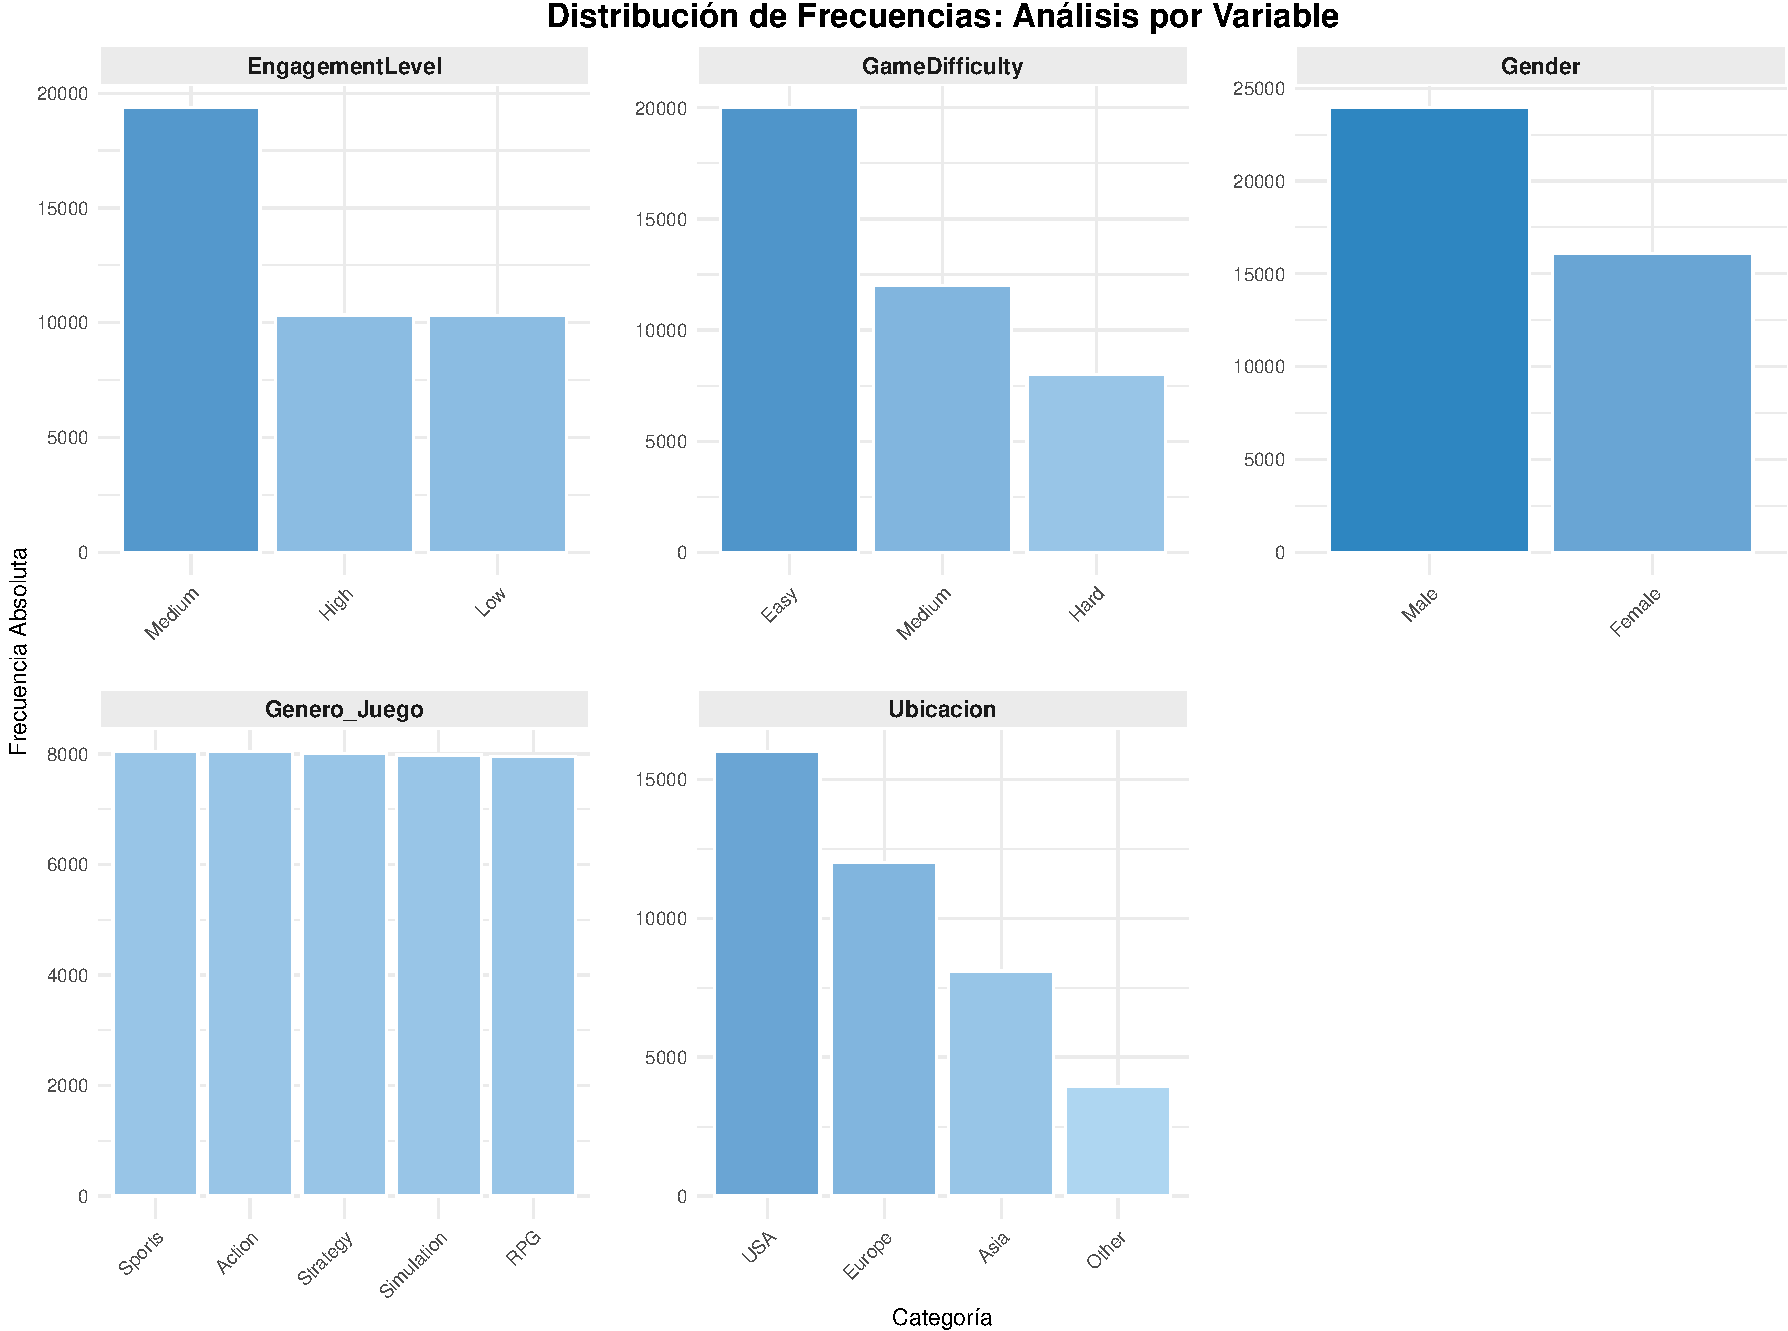
\includegraphics[width=0.9\linewidth,]{informe_files/figure-latex/grafica_frecuencias_libres-1} \end{center}

\subsection{Limpieza de datos}

Para asegurar que el análisis sea confiable, se realizó un proceso de
depuración sobre el dataset original:

\begin{itemize}
  \item{Tratamiento de Valores Nulos (NAs): Se identificaron los valores ausentes para asegurar que los cálculos de correlación se realicen sobre pares completos de datos, evitando sesgos en los estimadores. Lo que dio por resultado que el dataset no presenta valores nulos.} 
  \item{Detección de Duplicados e Inconsistencias: Se detectaron registros redundantes y de sintaxis o tipos de datos inconsistentes que dificultarían la lectura por parte de los algoritmos de R. El resultado fue que el dataset no presenta duplicados ni inconsistencias.} 
  \item{Normalización de Variables: Se verificó que las variables numéricas mantuvieran una estructura coherente para facilitar el cálculo de los momentos centrales y los estadísticos de dispersión. Se obtuvo que el dataset no necesita normalización de variables ya que estas cumplen con la sintaxis necesaria.}
  \item{Detección de Valores Atípicos: Se verifico que no hubiera valores atípicos que afecten la media. Lo que dio por resultado que la variable In Game Purchases contiene 8041 valores atípicos, ya que es una variable que no se toma en cuenta en la investigación no afecta el análisis.}
\end{itemize}

\chapter{Análisis de Resultados}

\{\small Este capítulo presenta los resultados obtenidos al aplicar las
metodologías descritas en el capítulo anterior, así como del análisis
estadístico descriptivo de las variables estudiadas y las ventajas y
desventajas al aplicar dichos tests.\}

\section{Presentación de resultados 1}

Descripción\\

\section{Presentación de resultados 2}

Descripción\\

\section{Presentación de resultados n}

Descripción\\

\chapter{Conclusiones y Recomendaciones}

\textbf{1.-} Conclusion 1 del trabajo de investigación.\\

\textbf{Recomendación} Recomendación 1 del trabajo de investigación.\\

\textbf{2.-} Conclusion 2 del trabajo de investigación.\\

\textbf{Recomendación} Recomendación 2 del trabajo de investigación.\\

\textbf{n.-} Conclusion n del trabajo de investigación.\\

\textbf{Recomendación} Recomendación n del trabajo de investigación.\\

\appendix
\renewcommand{\thechapter}{\Alph{chapter}}

\chapter{Anexo A}

\chapter{Anexo B}

\chapter{Anexo C}

%%%%%%%%%%%%%%%%%%%%%%%%%%%%%%%%%%%%%%%%%%%%%%%%%%%%%
%                   REFERENCIAS                     %
%%%%%%%%%%%%%%%%%%%%%%%%%%%%%%%%%%%%%%%%%%%%%%%%%%%%%
% Mantenemos la estructura natbib de tu plantilla
\renewcommand{\bibname}{Lista de Referencias}
\bibliographystyle{apalike} 
\bibliography{bibliografia.bib} 

%%%%%%%%%%%%%%%%%%%%%%%%%%%%%%%%%%%%%%%%%%%%%%%%%%%%%
%                   APÉNDICES                       %
%%%%%%%%%%%%%%%%%%%%%%%%%%%%%%%%%%%%%%%%%%%%%%%%%%%%%

\end{document}
